
Como dijimos anteriormente, el algoritmo tiene una complejidad de $\Theta(n + m)$. El algoritmo no tiene peor o mejor caso propiamente dichos (dado que es $\Theta(n + m)$ para todos los casos), pero veremos que, tomando $n$ fijo y moviendo $m$, podemos hacer variar el tiempo que toma el algoritmo.



\begin{figure}[H]
 \centering
	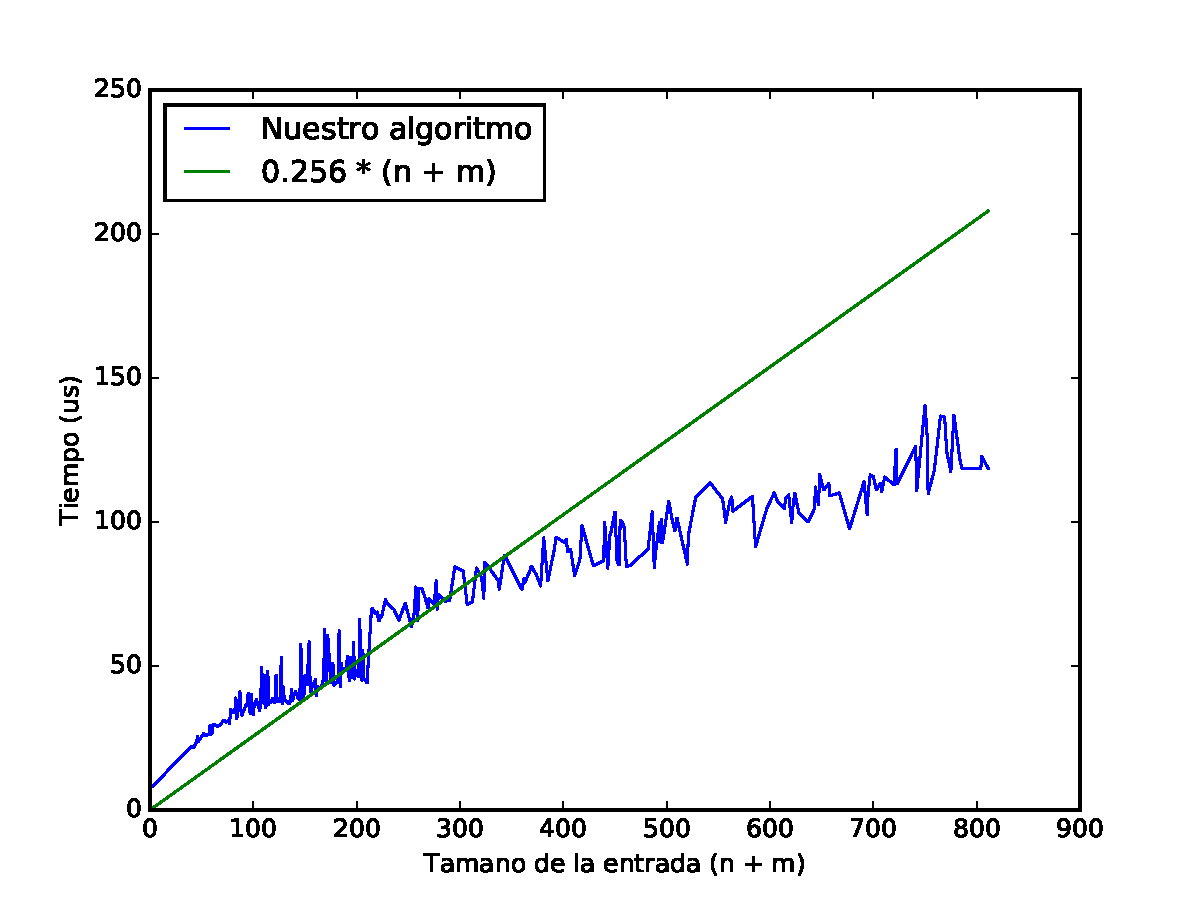
\includegraphics[width=0.8\textwidth]{img/exp/problema1-promedio.pdf}
	\caption{\footnotesize Tiempo que toma el algoritmo en $\mu$s para una entrada de tamaño $n + m$. $m$ al azar entre $n-1$ y $\frac{n(n-1)}{2}$.}
	\label{fig:problema1-promedio}
\end{figure}

Como se observa, la implementación tiene complejidad lineal sobre $n + m$, como era esperado.

Para confirmarlo, usamos el gráfico de la funcion $\frac{T(n + m)}{n + m}$, donde $T$ es el tiempo que tarda el algoritmo para la entrada de tamaño dado.
Si vemos que converge a una constante, estaremos en el caso exacto de la definción de $\Theta(f(n))$.

\begin{figure}[H]
 \centering
	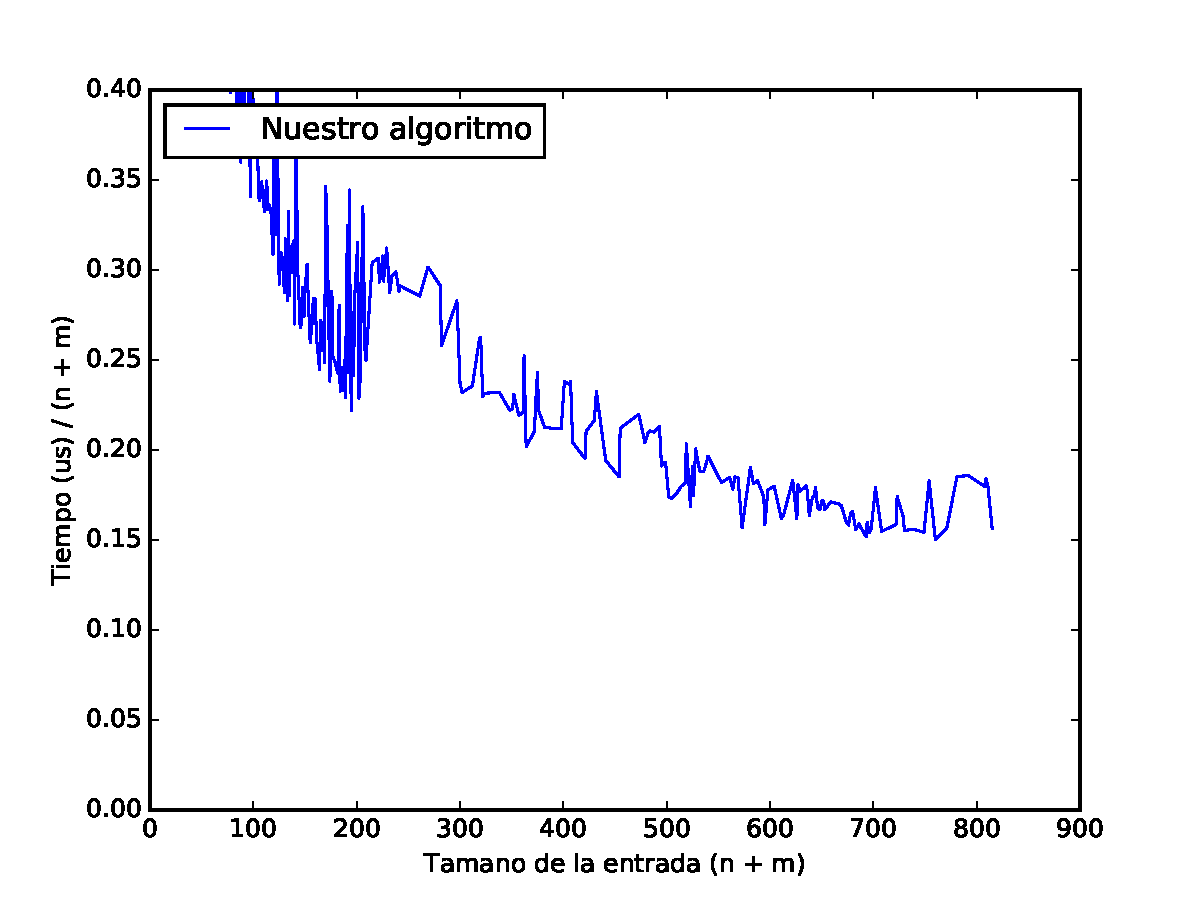
\includegraphics[width=0.8\textwidth]{img/exp/problema1-promedio2.pdf}
	\caption{\footnotesize Tiempo que toma el algoritmo en $\mu$s dividido $n + m$ para una entrada de tamaño $n + m$.  $m$ al azar entre $n-1$ y $\frac{n(n-1)}{2}$}
	\label{fig:problema1-promedio2}
\end{figure}

El ruido del gráfico se debe a que la escala es otra y distorciona las distancias entre los puntos. Sin embargo, se puede observar que converge a una constante, como era esperado.


Como habiamos dicho anteriormente, aunque el algoritmo es $\Theta(n + m)$, podemos ver casos particulares del algoritmo, en el que $n$ está fijo y movemos $m$ y ver como se comporta el algoritmo.

Primero veamos el caso en el que $m \in O(n)$. Esperaríamos que el algoritmo aquí tenga una complejidad de $O(n + m) = O(n + n) = O(n)$. Esto fue confirmado experimentalmente, como se muestra a continuación.

\begin{figure}[H]
 \centering
	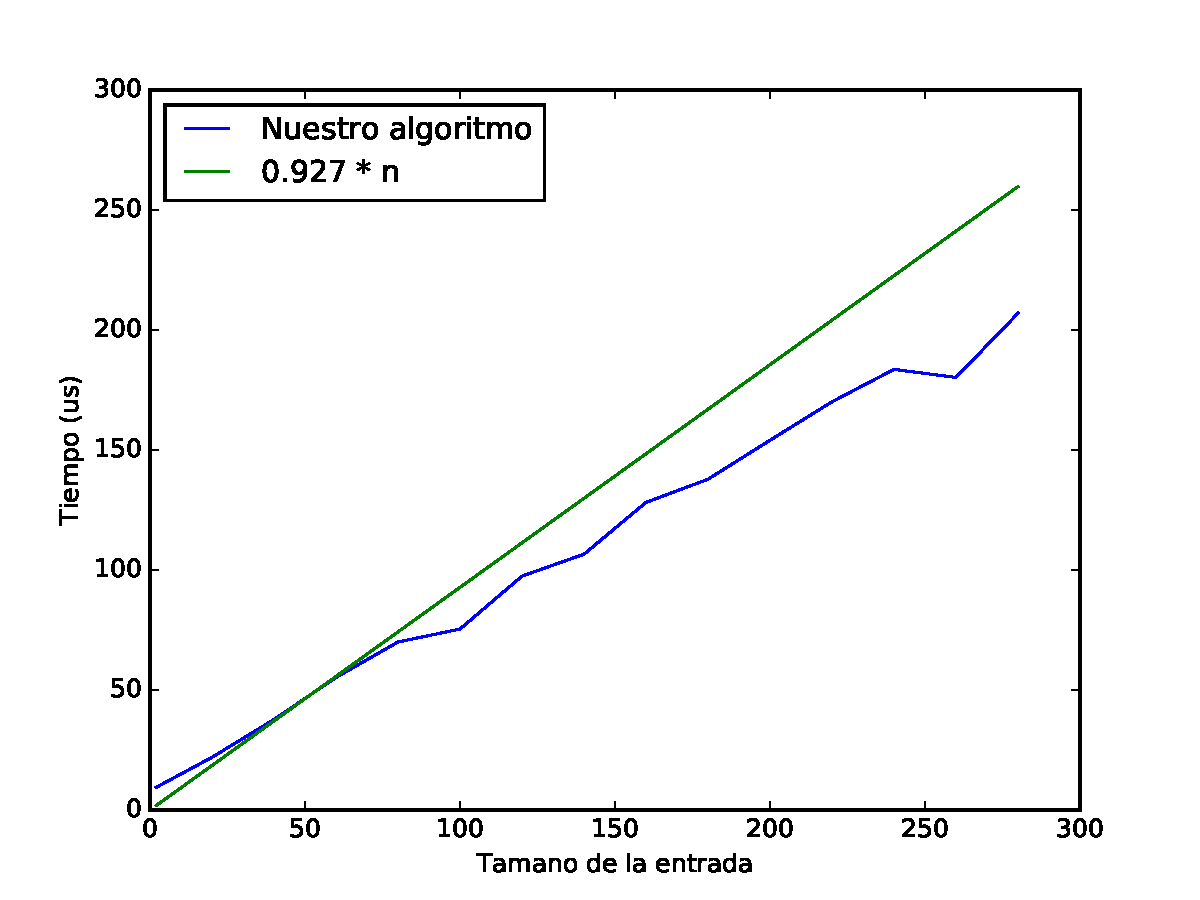
\includegraphics[width=0.8\textwidth]{img/exp/problema1-mejor.pdf}
	\caption{\footnotesize Tiempo que toma el algoritmo en $\mu$s para una entrada de tamaño $n$ ($m \in O(n))$.}
	\label{fig:problema1-mejor}
\end{figure}


Ahora veamos el caso en el que $m \in O(n^2)$. Esperaríamos que el algoritmo aquí tenga una complejidad de $O(n + m) = O(n + n^2) = O(n^2)$. Esto fue, nuevamente, confirmado experimentalmente.

\begin{figure}[H]
 \centering
	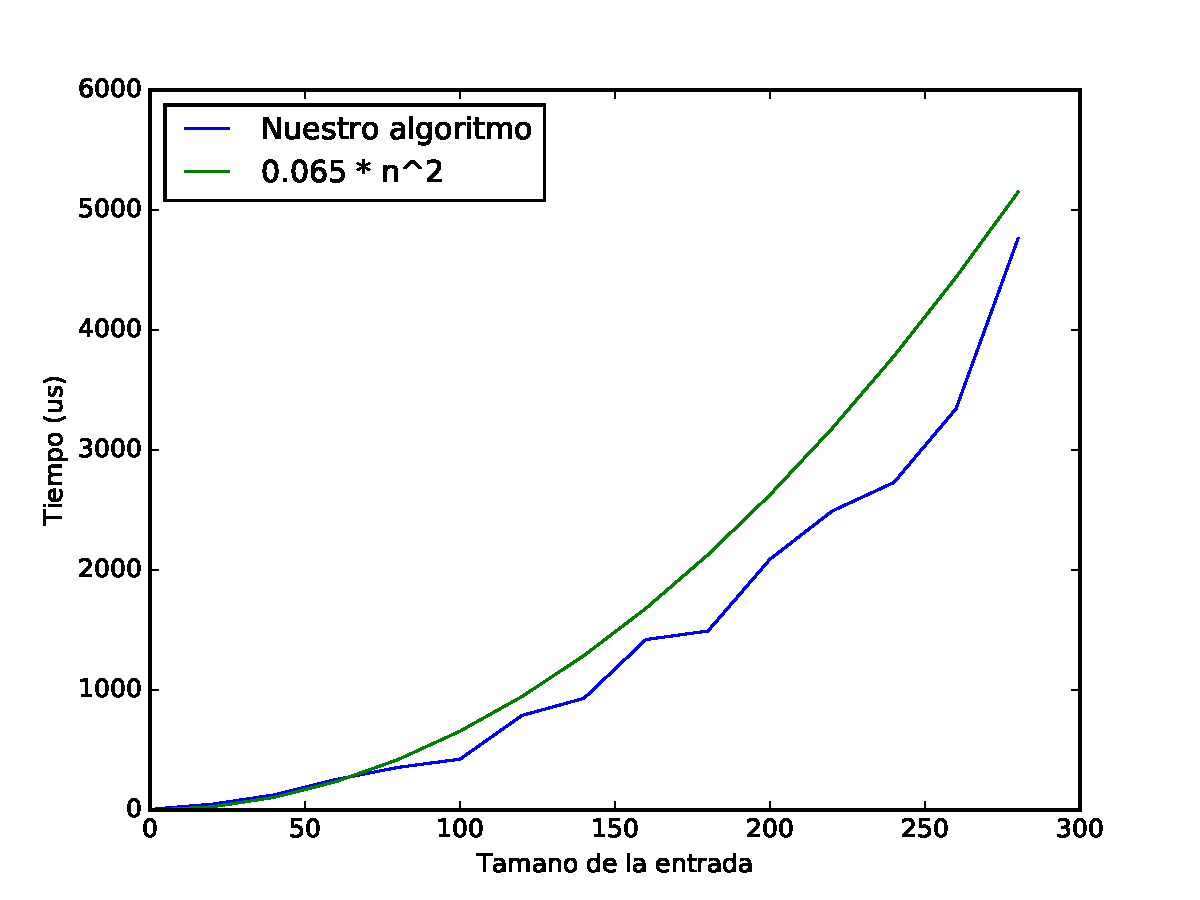
\includegraphics[width=0.8\textwidth]{img/exp/problema1-peor.pdf}
	\caption{\footnotesize Tiempo que toma el algoritmo en $\mu$s para una entrada de tamaño $n$ ($m \in O(n^2))$.}
	\label{fig:problema1-peor}
\end{figure}


\subsubsection{M\'etodo de experimentación}

Para la experimentación general del algoritmo, es decir, la verificación de que su complejidad era de $\Theta(n+m)$, generabamos distintos grafos al azar ($n$ al azar y $m$ elegido al azar tal que quede conexo).

En los casos particulares, dado $n$ fijo, tomamos $m = n - 1$ para el primer experimento y $m = \frac{n (n - 1)}{2}$ en el segundo experimento.

Para la generación al azar de grafos utilizamos el algoritmo descripto en el apéndice. 
